\newcommand{\componentA}{0.88}
\newcommand{\componentB}{0.96}
\newcommand{\componentC}{0.997}

\definecolor{motivation}{rgb}{\componentA, \componentB, \componentC}
\definecolor{building}{rgb}{  \componentB, \componentC, \componentA}
\definecolor{basics}{rgb}{    \componentB, \componentA, \componentC}
\definecolor{lists}{rgb}{     \componentA, \componentC, \componentB}
\definecolor{errors}{rgb}{    \componentC, \componentA, \componentB}
\definecolor{templates}{rgb}{ \componentC, \componentB, \componentA}
\definecolor{exercises}{rgb}{ \componentA, \componentB, \componentC}

\newcommand{\bgcolor}{Purple} % this should be renewed below

%%%%%%%%%%%%%%%%%%%%%%%%%%%%%%%%%%%%%%%%%%%%%%%%%%%%%%%%%%%%%%%
%%%%%%%%%%%%%%%%%%%%%%%%%%%%%%%%%%%%%%%%%%%%%%%%%%%% Motivation

% background color pre
{
\setbeamercolor{background canvas}{bg=motivation}
\renewcommand{\bgcolor}{motivation}

\section{Motivation}
\begin{frame}
  \vspace{25mm}
  \begin{center}
    \Huge{Part 1:\\Motivation}
  \end{center}
\end{frame}

\subsection{Observations}
\begin{frame}[fragile]
  \frametitle{Observations}
  \vspace{3mm}
  
\end{frame}

\subsection{Why \LaTeX?}
\begin{frame}[fragile]
  \frametitle{Why \LaTeX?}
  \vspace{3mm}
  
\end{frame}

\subsection{What is \LaTeX?}
\begin{frame}[fragile]
  \frametitle{What is \LaTeX?}
  \vspace{3mm}
  
\end{frame}

\subsection{Styles}
\begin{frame}[fragile]
  \frametitle{What is \LaTeX? \subpart{Styles}}
  \vspace{3mm}
  
\end{frame}

% background color post
}

%%%%%%%%%%%%%%%%%%%%%%%%%%%%%%%%%%%%%%%%%%%%%%%%%%%%%%%%%%%%%%%
%%%%%%%%%%%%%%%%%%%%%%%%%%%%%%%%%%%%%%%%%%%%%% Building the PDF

% background color pre
{
\setbeamercolor{background canvas}{bg=building}
\renewcommand{\bgcolor}{building}

\section{Building the PDF}
\begin{frame}
  \vspace{25mm}
  \begin{center}
    \Huge{Part 2:\\Building the PDF}
  \end{center}
\end{frame}

\subsection{Commandline}
\begin{frame}[fragile]
  \frametitle{Commandline}
  \vspace{3mm}
  
\end{frame}

\subsection{Overleaf}
\begin{frame}[fragile]
  \frametitle{Overleaf}
  \vspace{3mm}
  
\end{frame}

\subsection{Make}
\begin{frame}[fragile]
  \frametitle{Make}
  \vspace{3mm}
  
\end{frame}

\subsection{GIT}
\begin{frame}[fragile]
  \frametitle{GIT}
  \vspace{3mm}
  
\end{frame}

% background color post
}

%%%%%%%%%%%%%%%%%%%%%%%%%%%%%%%%%%%%%%%%%%%%%%%%%%%%%%%%%%%%%%%
%%%%%%%%%%%%%%%%%%%%%%%%%%%%%%%%%%%%%%%%%%%%%%%%%%%%%%%% Basics

% background color pre
{
\setbeamercolor{background canvas}{bg=basics}
\renewcommand{\bgcolor}{basics}

\section{Basics}
\begin{frame}
  \vspace{25mm}
  \begin{center}
    \Huge{Part 3:\\Basics}
  \end{center}
\end{frame}

\subsection{Overall Structure}
\begin{frame}[fragile]
  \frametitle{Overall Structure}
  \vspace{3mm}
  
\end{frame}

\subsection{Formatting}
\begin{frame}[fragile]
  \frametitle{Formatting}
  \vspace{18mm}
  
  \begin{tikzpicture}[remember picture,overlay]
    \newcommand{\height}[0]{36mm}
    \newcommand{\dist}[0]{5mm}
    
    \tikzstyle{dedge} = [thick,->,>=stealth,draw=black]
    
    \node[rectangle,thick,anchor=east,draw,minimum height=\height] (code) at ([xshift=-\dist]current page.center) {
      \begin{minipage}{5cm}
        \begin{minted}{latex}
normal \\
\textbf{bold} \\
\textsl{slanted} \\
\textit{italics} \\
\texttt{teletype} \\
\textsl{serif free} \\
\underline{underline}
        \end{minted}
      \end{minipage}
    };
    
    \node[rectangle,thick,anchor=west,draw,minimum height=\height] (output) at ([xshift=\dist]current page.center) {
      \begin{minipage}{5cm}
        normal \\
        \textbf{bold} \\
        \textsl{slanted} \\
        \textit{italics} \\
        \texttt{teletype} \\
        \textsl{serif free} \\
        \underline{underline}
      \end{minipage}
    };
    
    \draw[dedge] (code)->(output);
  \end{tikzpicture}
\end{frame}

\subsection{Text Size}
\begin{frame}[fragile]
  \frametitle{Text Size}
  \vspace{8mm}
  
  \begin{tikzpicture}[remember picture,overlay]
    \newcommand{\height}[0]{50mm}
    \newcommand{\dist}[0]{5mm}
    
    \tikzstyle{dedge} = [thick,->,>=stealth,draw=black]
    
    \node[rectangle,thick,anchor=east,draw,minimum height=\height] (code) at ([xshift=-\dist]current page.center) {
      \begin{minipage}{6cm}
        \begin{minted}[breaklines]{latex}
\tiny{Sample text}
\scriptsize{Sample text}
\footnotesize{Sample text}
\small{Sample text}
\normalsize{Sample text}
\large{Sample text}
\Large{Sample text}
\LARGE{Sample text}
\huge{Sample text}
\Huge{Sample text}
        \end{minted}
      \end{minipage}
    };
    
    \node[rectangle,thick,anchor=west,draw,minimum height=\height] (output) at ([xshift=\dist]current page.center) {
      \begin{minipage}{6cm}
        \tiny{Sample text}
        \scriptsize{Sample text}
        \footnotesize{Sample text}
        \small{Sample text}
        \normalsize{Sample text}
        \large{Sample text}
        \Large{Sample text}
        \LARGE{Sample text}
        \huge{Sample text}
        \Huge{Sample text}
      \end{minipage}
    };
    
    \draw[dedge] (code)->(output);
  \end{tikzpicture}
\end{frame}

\subsection{Listings}
\begin{frame}[fragile]
  \frametitle{Listings}
  \vspace{3mm}
  
\end{frame}

\subsubsection{Itemization}
\begin{frame}[fragile]
  \frametitle{Listings \subpart{Itemization}}
  \vspace{18mm}
  
  \begin{tikzpicture}[remember picture,overlay]
    \newcommand{\height}[0]{36mm}
    \newcommand{\dist}[0]{5mm}
    
    \tikzstyle{dedge} = [thick,->,>=stealth,draw=black]
    
    \node[rectangle,thick,anchor=east,draw,minimum height=\height] (code) at ([xshift=-\dist]current page.center) {
      \begin{minipage}{5cm}
        \begin{minted}{latex}
Programming languages:
\begin{itemize}
  \item Rust
  \item Elixir
  \item Python
  \item \LaTeX ?
\end{itemize}
        \end{minted}
      \end{minipage}
    };
    
    \node[rectangle,thick,anchor=west,draw,minimum height=\height] (output) at ([xshift=\dist]current page.center) {
      \begin{minipage}{5cm}
        Programming languages:
        \begin{itemize}
          \item Rust
          \item Elixir
          \item Python
          \item \LaTeX ?
        \end{itemize}
      \end{minipage}
    };
    
    \draw[dedge] (code)->(output);
  \end{tikzpicture}
\end{frame}

\subsubsection{Enumerations}
\begin{frame}[fragile]
  \frametitle{Listings \subpart{Enumerations}}
  \vspace{18mm}
  
  \begin{tikzpicture}[remember picture,overlay]
    \newcommand{\height}[0]{36mm}
    \newcommand{\dist}[0]{5mm}
    
    \tikzstyle{dedge} = [thick,->,>=stealth,draw=black]
    
    \node[rectangle,thick,anchor=east,draw,minimum height=\height] (code) at ([xshift=-\dist]current page.center) {
      \begin{minipage}{5cm}
        \begin{minted}{latex}
Programming languages:
\begin{enumerate}
  \item Rust
  \item Elixir
  \item Python
  \item \LaTeX ?
\end{enumerate}
        \end{minted}
      \end{minipage}
    };
    
    \node[rectangle,thick,anchor=west,draw,minimum height=\height] (output) at ([xshift=\dist]current page.center) {
      \begin{minipage}{5cm}
        Programming languages:
        \begin{enumerate}
          \item Rust
          \item Elixir
          \item Python
          \item \LaTeX ?
        \end{enumerate}
      \end{minipage}
    };
    
    \draw[dedge] (code)->(output);
  \end{tikzpicture}
\end{frame}

\subsection{References}
\begin{frame}[fragile]
  \frametitle{References}
  \vspace{3mm}
  
\end{frame}

\subsection{Colors}
\begin{frame}[fragile]
  \frametitle{Colors}
  \vspace{3mm}
  
\end{frame}

\subsection{Tables}
\begin{frame}[fragile]
  \frametitle{Tables}
  \vspace{3mm}
  
\end{frame}

\subsection{Including Visuals}
\begin{frame}[fragile]
  \frametitle{Including Visuals}
  \vspace{3mm}
  When it comes to visual aids, \LaTeX\ supports a number of different types.
  
  \begin{center}
    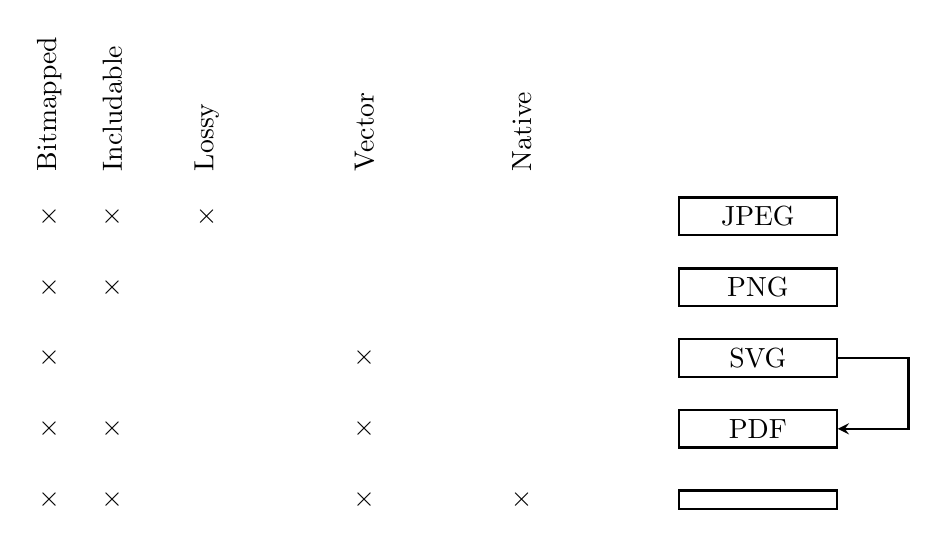
\begin{tikzpicture}[]
      \newcommand{\bitmapX}[0]{0mm}
      \newcommand{\lossyX}[0]{20mm}
      \newcommand{\vectorX}[0]{40mm}
      \newcommand{\stylableX}[0]{60mm}
      \newcommand{\includableX}[0]{8mm}
      \newcommand{\formatX}[0]{90mm}
      \newcommand{\convertX}[0]{120mm}
      
      \newcommand{\stepY}[0]{-9mm}
      
      \tikzstyle{label} = []
      \tikzstyle{format} = [
        rectangle,
        thick,
        draw,
        minimum width=2cm,
      ]
      
      \tikzstyle{dedge} = [thick,->,>=stealth,draw=black]
      
      \node[label,anchor=south] () at (\bitmapX, -0.5*\stepY) {\rotatebox{90}{Bitmapped}};
      \node[label,anchor=south] () at (\lossyX, -0.5*\stepY) {\rotatebox{90}{Lossy}};
      \node[label,anchor=south] () at (\vectorX, -0.5*\stepY) {\rotatebox{90}{Vector}};
      \node[label,anchor=south] () at (\stylableX, -0.5*\stepY) {\rotatebox{90}{Native}};
      \node[label,anchor=south] () at (\includableX, -0.5*\stepY) {\rotatebox{90}{Includable}};
      
      \node[label] () at (\bitmapX, 0*\stepY) {$\times$};
      \node[label] () at (\lossyX, 0*\stepY) {$\times$};
      \node[label] () at (\includableX, 0*\stepY) {$\times$};
      \node[format] () at (\formatX, 0*\stepY) {JPEG};
      
      \node[label] () at (\bitmapX, 1*\stepY) {$\times$};
      \node[label] () at (\includableX, 1*\stepY) {$\times$};
      \node[format] () at (\formatX, 1*\stepY) {PNG};
      
      \node[label] () at (\bitmapX, 2*\stepY) {$\times$};
      \node[label] () at (\vectorX, 2*\stepY) {$\times$};
      \node[format] (svg) at (\formatX, 2*\stepY) {SVG};
      
      \node[label] () at (\bitmapX, 3*\stepY) {$\times$};
      \node[label] () at (\vectorX, 3*\stepY) {$\times$};
      \node[label] () at (\includableX, 3*\stepY) {$\times$};
      \node[format] (pdf) at (\formatX, 3*\stepY) {PDF};
      
      \node[label] () at (\bitmapX, 4*\stepY) {$\times$};
      \node[label] () at (\vectorX, 4*\stepY) {$\times$};
      \node[label] () at (\stylableX, 4*\stepY) {$\times$};
      \node[label] () at (\includableX, 4*\stepY) {$\times$};
      \node[format] () at (\formatX, 4*\stepY) {\TikZ};
      
      \draw[dedge] (svg)
                 --([xshift=-\stepY]svg.east)
                 --([xshift=-\stepY]pdf.east)
                 --(pdf);
    \end{tikzpicture}
  \end{center}
\end{frame}

\subsubsection{PDF Graphics}
\begin{frame}[fragile]
  \frametitle{Including Visuals \subpart{PDF Graphics}}
  \vspace{3mm}
  
\end{frame}

\subsubsection{SVG Graphics}
\begin{frame}[fragile]
  \frametitle{Including Visuals \subpart{SVG Graphics}}
  \vspace{3mm}
  
\end{frame}

\subsubsection{Bitmapped Graphics}
\begin{frame}[fragile]
  \frametitle{Including Visuals \subpart{Bitmapped Graphics}}
  \vspace{3mm}
  
\end{frame}

\subsection{Figures}
\begin{frame}[fragile]
  \frametitle{Figures}
  \vspace{3mm}
  
\end{frame}

\subsection{Notes}
\begin{frame}[fragile]
  \frametitle{Notes}
  \vspace{3mm}
  
\end{frame}

\subsection{Code Inclusion}
\begin{frame}[fragile]
  \frametitle{Code Inclusion}
  \vspace{3mm}
  
\end{frame}

\subsection{URLs}
\begin{frame}[fragile]
  \frametitle{URLs}
  \vspace{3mm}
  
\end{frame}

% background color post
}

%%%%%%%%%%%%%%%%%%%%%%%%%%%%%%%%%%%%%%%%%%%%%%%%%%%%%%%%%%%%%%%
%%%%%%%%%%%%%%%%%%%%%%%%%%%%%%%%%%%%%%%%%%%%%%%%%%%%%%%%% Lists

% background color pre
{
\setbeamercolor{background canvas}{bg=lists}
\renewcommand{\bgcolor}{lists}

\section{Lists}
\begin{frame}
  \vspace{25mm}
  \begin{center}
    \Huge{Part 4:\\Lists}
  \end{center}
\end{frame}

\subsection{Table of Contents}
\begin{frame}[fragile]
  \frametitle{Table of Contents}
  \vspace{3mm}
  
\end{frame}

\subsection{List of Figures}
\begin{frame}[fragile]
  \frametitle{List of Figures}
  \vspace{3mm}
  
\end{frame}

\subsection{List of Tables}
\begin{frame}[fragile]
  \frametitle{List of Tables}
  \vspace{3mm}
  
\end{frame}

\subsection{Bibliography}
\begin{frame}[fragile]
  \frametitle{Bibliography}
  \vspace{3mm}
  
\end{frame}

\subsection{Index}
\begin{frame}[fragile]
  \frametitle{Index}
  \vspace{3mm}
  
\end{frame}

% background color post
}

%%%%%%%%%%%%%%%%%%%%%%%%%%%%%%%%%%%%%%%%%%%%%%%%%%%%%%%%%%%%%%%
%%%%%%%%%%%%%%%%%%%%%%%%%%%%%%%%%%%%%%%%%%% Dealing with Errors

% background color pre
{
\setbeamercolor{background canvas}{bg=errors}
\renewcommand{\bgcolor}{errors}

\section{Dealing with Errors}
\begin{frame}
  \vspace{25mm}
  \begin{center}
    \Huge{Part 5:\\Dealing with Errors}
  \end{center}
\end{frame}

\subsection{Locating the Error}
\begin{frame}[fragile]
  \frametitle{Locating the Error}
  \vspace{3mm}
  
\end{frame}

\subsection{Googling the Error}
\begin{frame}[fragile]
  \frametitle{Googling the Error}
  \vspace{3mm}
  
\end{frame}

% background color post
}

%%%%%%%%%%%%%%%%%%%%%%%%%%%%%%%%%%%%%%%%%%%%%%%%%%%%%%%%%%%%%%%
%%%%%%%%%%%%%%%%%%%%%%%%%%%%%%%%%%%%%%%%%%%%%%%%%%%%% Templates

% background color pre
{
\setbeamercolor{background canvas}{bg=templates}
\renewcommand{\bgcolor}{templates}

\section{Templates}
\begin{frame}
  \vspace{25mm}
  \begin{center}
    \Huge{Part 6:\\Templates}
  \end{center}
\end{frame}

\subsection{Source}
\begin{frame}[fragile]
  \frametitle{Source}
  \vspace{3mm}
  
\end{frame}

\subsection{Reports}
\begin{frame}[fragile]
  \frametitle{Reports}
  \vspace{3mm}
  
\end{frame}

\subsection{Presentations}
\begin{frame}[fragile]
  \frametitle{Presentations}
  \vspace{3mm}
  
\end{frame}

% background color post
}

%%%%%%%%%%%%%%%%%%%%%%%%%%%%%%%%%%%%%%%%%%%%%%%%%%%%%%%%%%%%%%%
%%%%%%%%%%%%%%%%%%%%%%%%%%%%%%%%%%%%%%%%%%%%%%%%%%%%% Exercises

% background color pre
{
\setbeamercolor{background canvas}{bg=exercises}
\renewcommand{\bgcolor}{exercises}

\section{Exercises}
\begin{frame}
  \vspace{25mm}
  \begin{center}
    \Huge{Part 7:\\Exercises}
  \end{center}
\end{frame}

\subsection{Exercises}
\begin{frame}[fragile]
  \frametitle{Exercises}
  \vspace{3mm}
  \begin{enumerate}
    \descitem{New Project:} Create a new project (on Overleaf, GitHub or similar). Make sure that you have a report \LaTeX\ document that builds.
    \descitem{Report:} Pick any old report, and port it to \LaTeX. The point is not to go through the whole report, but rather to get a feel of (i) the effort needed to port an old report, and (ii) the perceived typographical quality per effort.
  \end{enumerate}
\end{frame}

% background color post
}

